
\chapter{Vysledky prace}

V tejto kapitole zhrnieme vysledky ktore nasa praca dosiahla.

Uz v predchadzajucich kappitolach sme sa stretli s niekolkymi prikladmi, napriklad ako si
program poradil s vkladanim do hairpinu - obrazok \ref{obr:insert_circle_hairpin}.

Na dalsom (obrazok \ref{obr:delete_insert_multibranch}) simulujeme mazanie s naslednym vkladanim,
teda 2 k sebe inverzne operacie. Po zmazaní bazovych parov na hornej vetve molekuly, sa nam vsetky
neparove bazy zliali a vytvorili jednu loop. Nasledne po opatovnom vlozeni bazovych parov (pre lepsie
zviditelnenie sme ich oznacili "I"), vznikla struktura velmi podobna predchadzajucej.

Obrazok ma za ciel ukazat, ze vieme znovu nakreslit povodnu strukturu iba s malymi zmenamy v pozicii
nukleotidov (vysledne loopy su trochu plytsie ako povodne).

Rovnako obrazok \ref{obr:delete_insert_multibranch_loop} rekonstruuje vetvenie sa stromu. Ako je vidiet,
v tomto obrazku je uz viac rozdielov, vychylenie je celkom badatelne.

Na takto malych castiach bez velkych vetveni nam ani taketo zmeny nevadia. Pri velkych molekulach
ako ukazeme neskor problemy nastavaju.

\begin{figure}[H]
  \begin{subfigure}{0.3\textwidth}
%trim=left bottom right top
    \includegraphics[clip, trim=1cm 21cm 14cm 2.5cm, width=0.85\textwidth]{../img/alg-insert/2/multibranch-beg}
  \end{subfigure}
  \begin{subfigure}{0.3\textwidth}
%trim=left bottom right top
    \includegraphics[clip, trim=1cm 21cm 14cm 2.5cm, width=0.85\textwidth]{../img/alg-insert/2/multibranch-del}
  \end{subfigure}
  \begin{subfigure}{0.3\textwidth}
%trim=left bottom right top
    \includegraphics[clip, trim=1cm 21cm 14cm 2.5cm, width=0.85\textwidth]{../img/alg-insert/2/multibranch-del-ins}
  \end{subfigure}
  \caption{Inverzne operacie: rekonstrukcia stemu}
  \label{obr:delete_insert_multibranch}
\end{figure}


\begin{figure}[H]
  \begin{subfigure}{0.3\textwidth}
%trim=left bottom right top
    \includegraphics[clip, trim=1cm 21cm 14cm 2.5cm, width=0.85\textwidth]{../img/alg-insert/3/multibranch-beg}
  \end{subfigure}
  \begin{subfigure}{0.3\textwidth}
%trim=left bottom right top
    \includegraphics[clip, trim=0 0 0 15cm, width=0.85\textwidth]{../img/alg-insert/3/multibranch-del}
  \end{subfigure}
  \begin{subfigure}{0.3\textwidth}
%trim=left bottom right top
    \includegraphics[clip, trim=0 0 0 2cm, width=0.85\textwidth]{../img/alg-insert/3/multibranch-del-ins}
  \end{subfigure}
  \caption{Inverzne operacie: rekonstrukcia multibranch loop}
  \label{obr:delete_insert_multibranch_loop}
\end{figure}


Ako dalsie, testovali sme schopnost nasho algoritmu vizualizovat znamu podjednotku 16S ribozomalnej RNA
na zivocisnej risi. CRW databaza obsahuje 16 organizmov so znamou sekundarnou strukturou.

Ribozomalna RNA bola vybrata lebo je v centre zaujmu mnohych vyskumov a taktiez kvoli jej velkosti
a zlozitosti.

Nas vizualizacny test sme spustili na vsetky pary RNA, z ktorych sme ziskali 256 vizualizacii.

%Na zaciatku potrebujeme uviest, ze z celkoveho poctu 256 vizualizacii dopadlo 21 neuspechom pre rozne dovody.
%Tym hlavnym je 

Na obrazku \ref{obr:statistika_prekryvy} vidime pocty molekul s danym poctom prekryvov. 
Je ale niekolko typov molekul u ktorych sme nejake prekryvy cakali - napriklad, ak sme v nej
potrebovali prekreslit multibranch loop. Takuto zavislost nam vyjadruju dalsie dva grafy,
prvy - \ref{obr:statistika_prekryvy_s_rotaciami} nam ukazuje, ze ak program musel rotovat
a prekreslovat multibranch loopy, nedarilo sa mu najlepsie. Naopak, ak z prveho grafu
odoberieme molekuly, ktore museli pouzit rotacie - graf \ref{obr:statistika_prekryvy_bez_rotacii},
vidime, ze algoritmus sablonovej vizualizacie si viedol celkom dobre, prekryvy vznikali iba ojedinele.


\begin{figure}
  \includegraphics[width=1\textwidth]{../img/statistika/prekryvy-pocetmolekul}
  \caption{Počet prekryvov v testovaných molekulách}
  \label{obr:statistika_prekryvy}
\end{figure}


\begin{figure}
  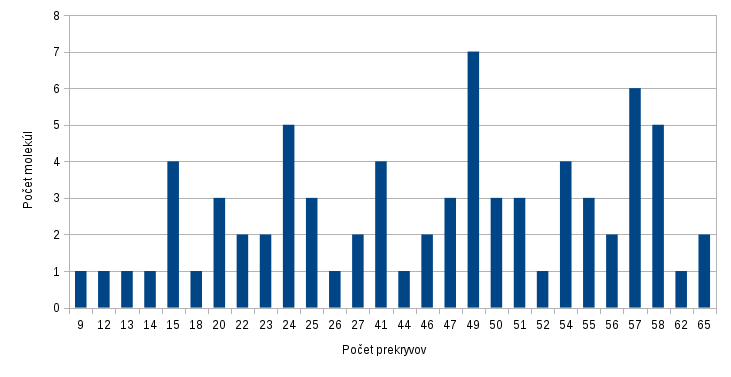
\includegraphics[width=1\textwidth]{../img/statistika/prekryvy-pocetmolekul-s-rotaciami}
  \caption{Počet prekryvov: molekuly ktore potrebovali prekreslit multibranch loop}
  \label{obr:statistika_prekryvy_bez_rotacii}
\end{figure}


\begin{figure}
  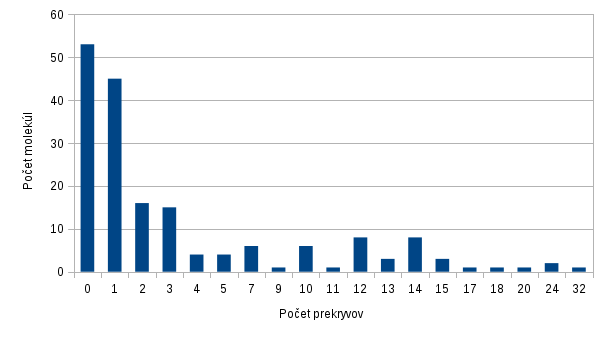
\includegraphics[width=1\textwidth]{../img/statistika/prekryvy-pocetmolekul-bez-rotacii}
  \caption{Počet prekryvov: molekuly bez prekreslovania multibranch loop}
  \label{obr:statistika_prekryvy_s_rotaciami}
\end{figure}

\begin{table}[b]
  \centering
  \begin{tabular}{l@{\hspace{1.5cm}}D{.}{,}{3.2}D{.}{,}{1.2}D{.}{,}{2.3}}
    \toprule
                                  & \mc{\textbf{Počet}}								& \mc{\textbf{Smerodajná}}		& \\
    \mc{\textbf{Vzdialenosť}}	    & \mc{\textbf{prekryvov}}	          & \mc{\textbf{odchýlka}}	    & \\
                                  & \mc{\textbf{(priemer)}}           &                            	& \\
    \midrule
    1.														&	5.13															&	1.64												& \\
    5.														&	13.38															&	9.57												&	\\
    10.														&	14.13															&	12.47												&	\\
    15.														&	15.25															&	0.66												&	\\
    \bottomrule
  \end{tabular}
\caption{Počty prekryvov v závislosti od tree-edit-distance vzdialenosti}
\label{tab:statistika_prekryvy}
\end{table}

Z tabulky \ref{tab:statistika_prekryvy} je vidiet, ze pocet prekryvov zavisi od poctu operacii vkladania
a mazania ktore v molekule musime urobit. Statistika pracuje s prvou, piatou, desiatou a patnastou najblizsou
molekulou z pohladu $tree-edit-distance$.

Zaujimavostou je, ze ako najvzdialenejsiu molekulu (v poradi patnastu) si vsetci vybrali molekulu od
jedneho konkretneho zastupcu $echinococcus\_granulosus$ a vzdialenost je $805,63$ s odchylkou $12,92$.

\section{Celkove vysledky}

V tejto kapitole uvedieme vygenerovane obrazky niektorych molekul a na nich ukazeme caste problemy,
ktore pri vizualizacii nastavali.

\subsection{Otacanie vetvy kvoli existujucej hrane}

Jednym prikladom za vsetky je molekula zivocicha $Tripedalia cystophora$ - meduzy.
Po tom, co sme dali molekulu nakreslit samu na seba vznikol problem, ze cela jedna
vetva molekuly sa otocila na jednu stranu. Je to sposobene existenciou bazoveho paru,
ktory je v povodnej molekule znazorneny dlhsou lomenou ciarou.

Kedze nas program vsetky vzdialenosti normalizuje a nasledne uklada bazy stemu na jednu priamku,
vznikaju obrazky podobne \ref{obr:chyba_otocenie_vetvy}.

\begin{figure}
  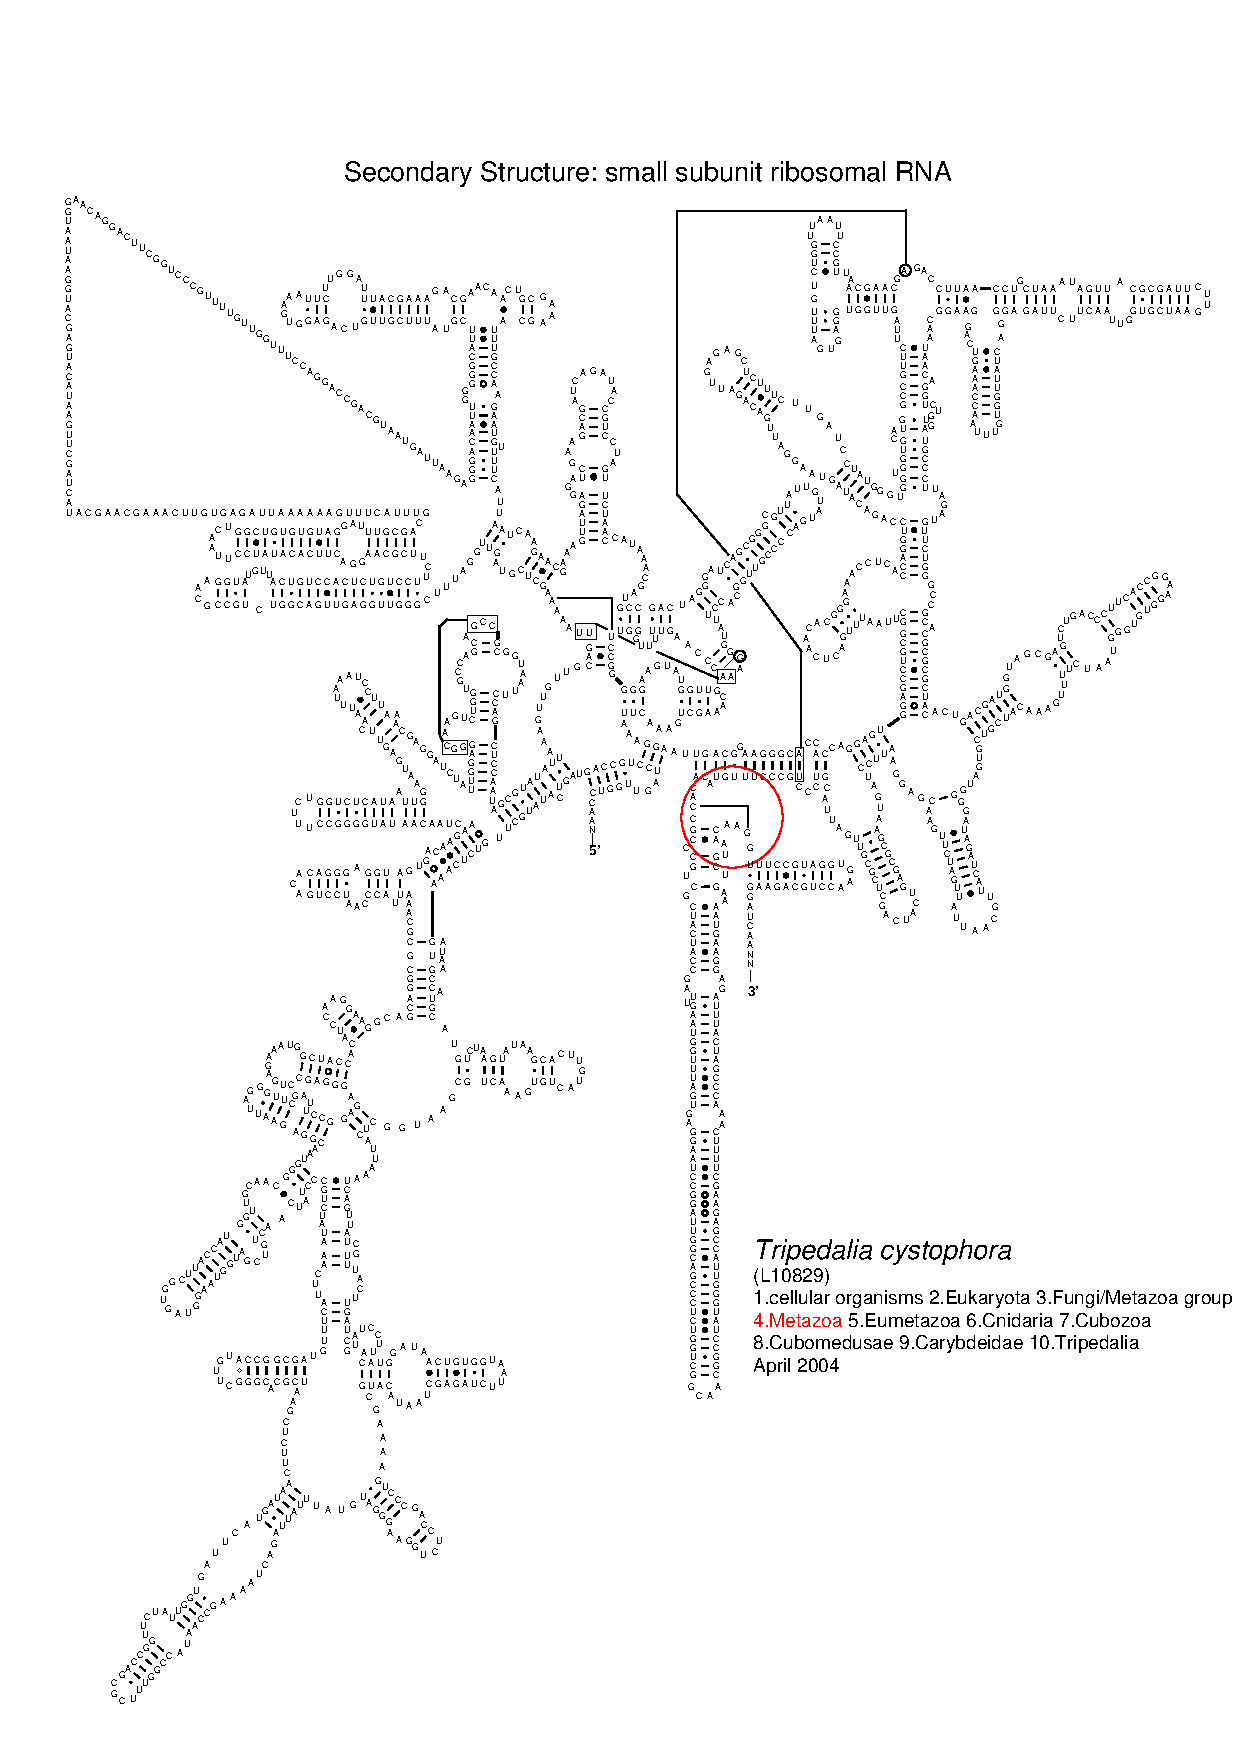
\includegraphics[width=0.45\textwidth]{../img/chyby/tripedalia_cystophora}
  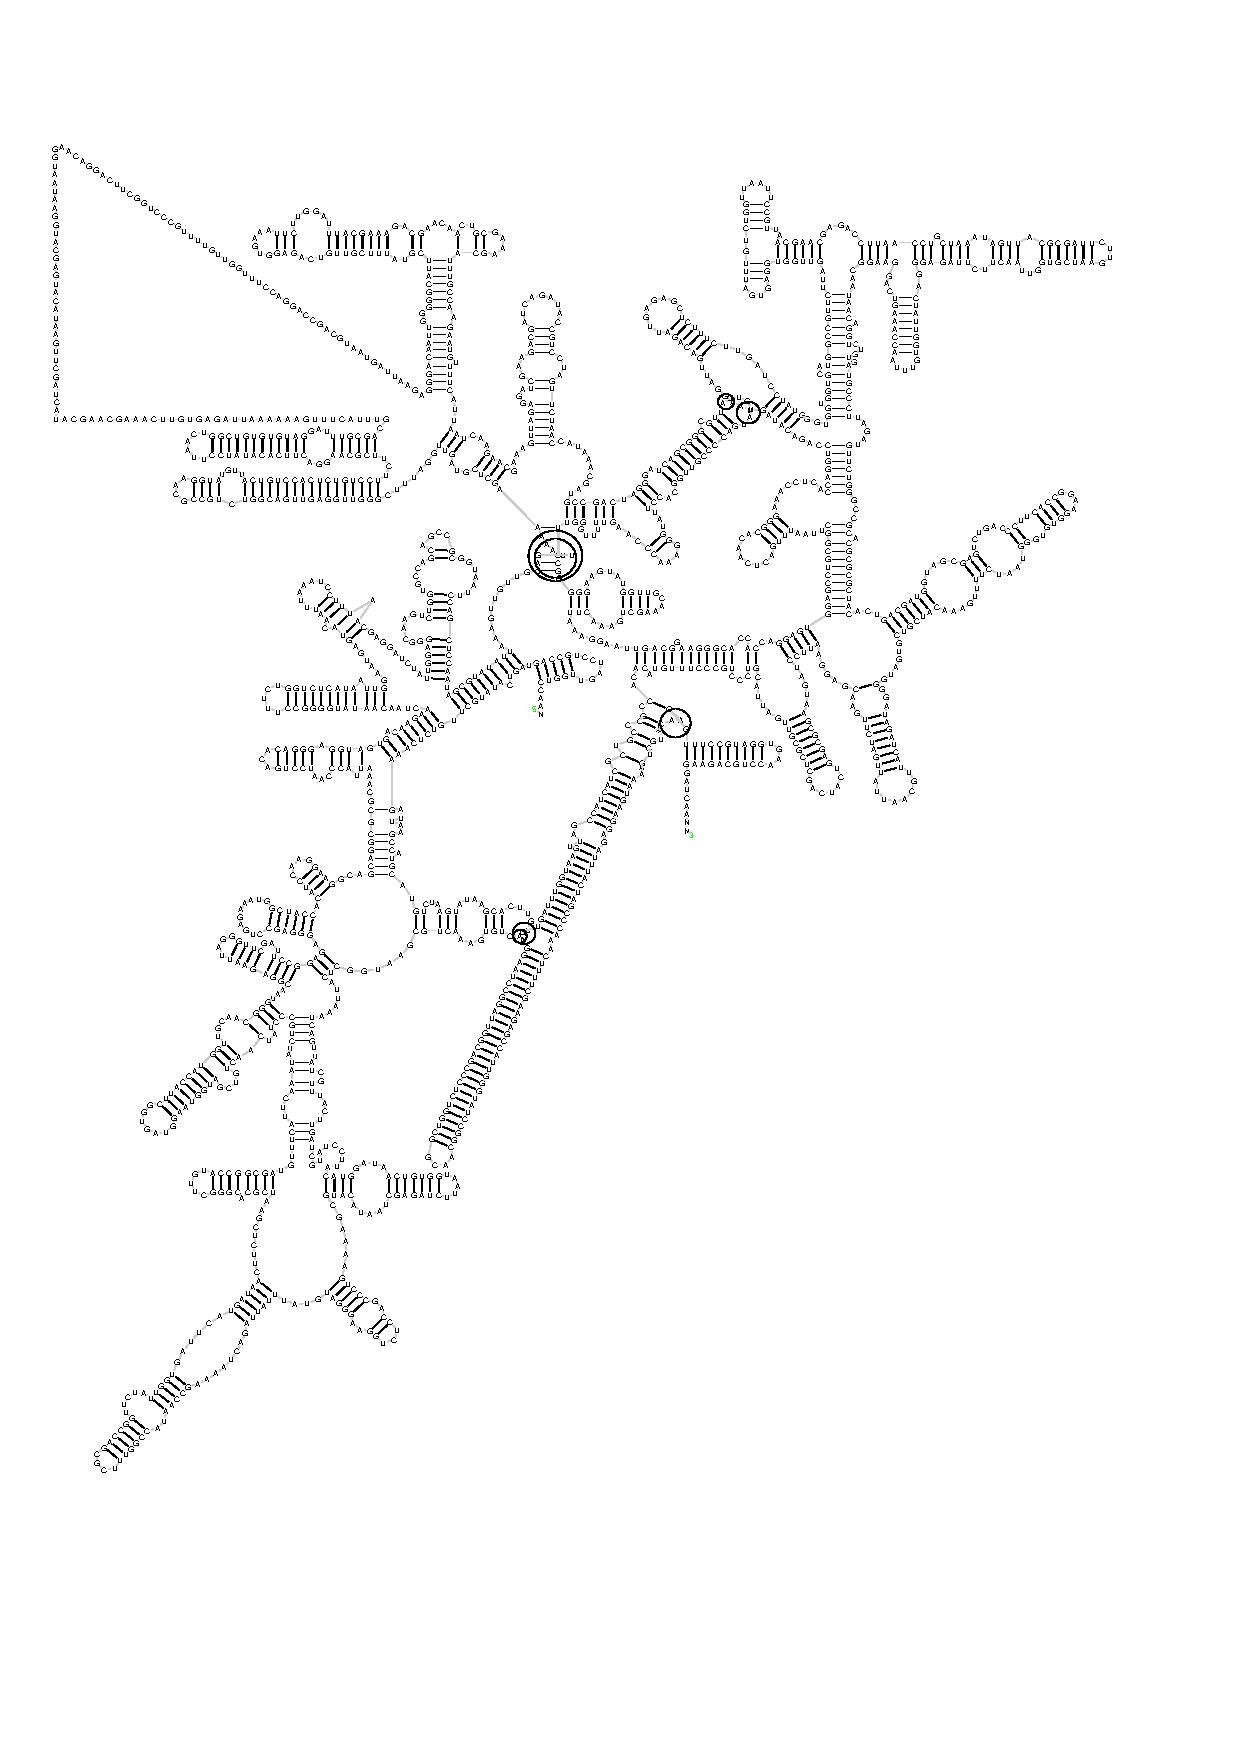
\includegraphics[width=0.45\textwidth]{../img/chyby/tripedalia_cystophora-tripedalia_cystophora}
  \caption{Chyba pri otoceni vetvy}
  \label{obr:chyba_otocenie_vetvy}
\end{figure}

\subsection{Rozlozenie baz na kruznicu}

Niekedy sa prekresleniu celej loop nevyhneme. Ak napriklad vkladame velmi velke mnozstvo baz na jedno
miesto, dochadza k problemom nacrtnutym na obrazku \ref{obr:chyba_rozlozenie_loopy}.

Na tomto konkretnom priklade je nakresleny stem, vo vnutri ktoreho je velka loop. Kvoli tomu,
ze chceme dodrziavat pravidla o kruznicovom tvare loopy, najdeme kruznicu dostatocne velku.
V tomto pripade az priliz velku.

Poznamka - vo vrchnej vetve ja taktiez znazornena kruznica, ale na rozdiel od spodnej obsahuje iba 2 vrcholy.

\begin{figure}[H]
%trim=left bottom right top
  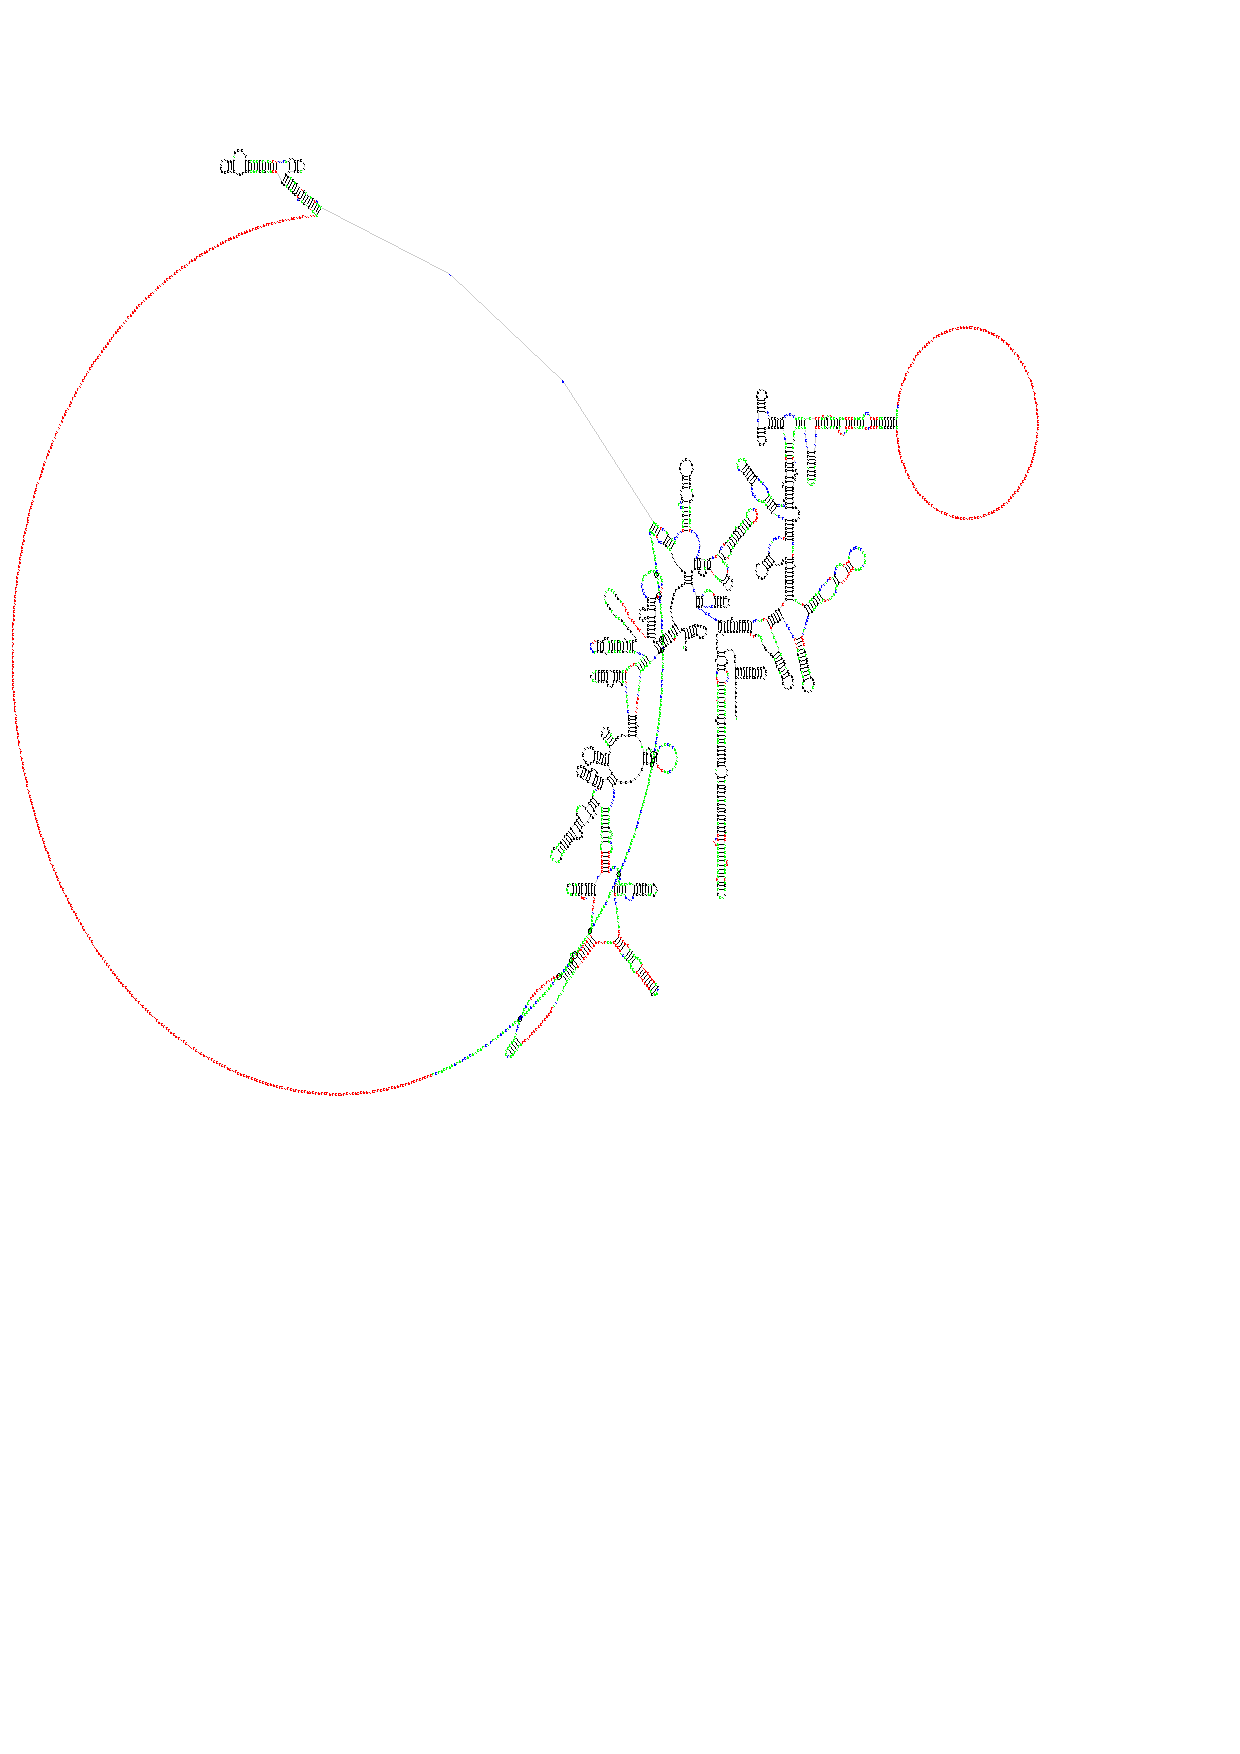
\includegraphics[clip, trim=0 10cm 3cm 2cm,width=0.8\textwidth]{../img/chyby/african_frog-echinococcus_granulosus}
  \caption{Chyba pri rozkladani baz na kruznicu}
  \label{obr:chyba_rozlozenie_loopy}
\end{figure}

\subsection{Otacanie vetvy kvoli prekreslovaniu multibranch loopy}

Ako uz aj graf na obrazku \ref{obr:statistika_prekryvy_bez_rotacii} ukazal,
prekreslovanie multibranch loopy a rotacie vsetkych vetiev sposobuje masivne prekryvy.

Pripajame jeden priklad na obrazku \ref{obr:chyba_rotacia_multibranch}. Miesto vlavo dolu, kde zacinaju
bazy sa sfarbovat na hnedo, je multibranch loop, ktoru sme potrebovali z dovodu vlozenej novej vetvy
(oznacena cerveno) prekreslit.

Vysledok je taky, ze vsetky vetvy sme ulozili na kruznicu a pootacali do vhodneho smeru a tym vzniklo
vela prekryvov.

Na obrazku je vidiet este jednu vec, oznacene krizenia vo vyslednom obrazku vlavo hore.
V kapitole o upravach multibranch loop sme spominali, ze prekresleniu celej loopy sa snazime
vyhnut ak to ide. Predpokladame, ze ak je baz vela a zmeny male, bazy trochu poposuvame aby sa
novy vrchol zmestil medzi ne, alebo prave naopak ich roztiahneme, aby sme vyplnili medzeru po starom.
Kvoli tomu vyzera tato struktura tak pomiesane a kvoli tomu na tomto mieste vznikaju dalsie prekryvy.

\begin{figure}
  %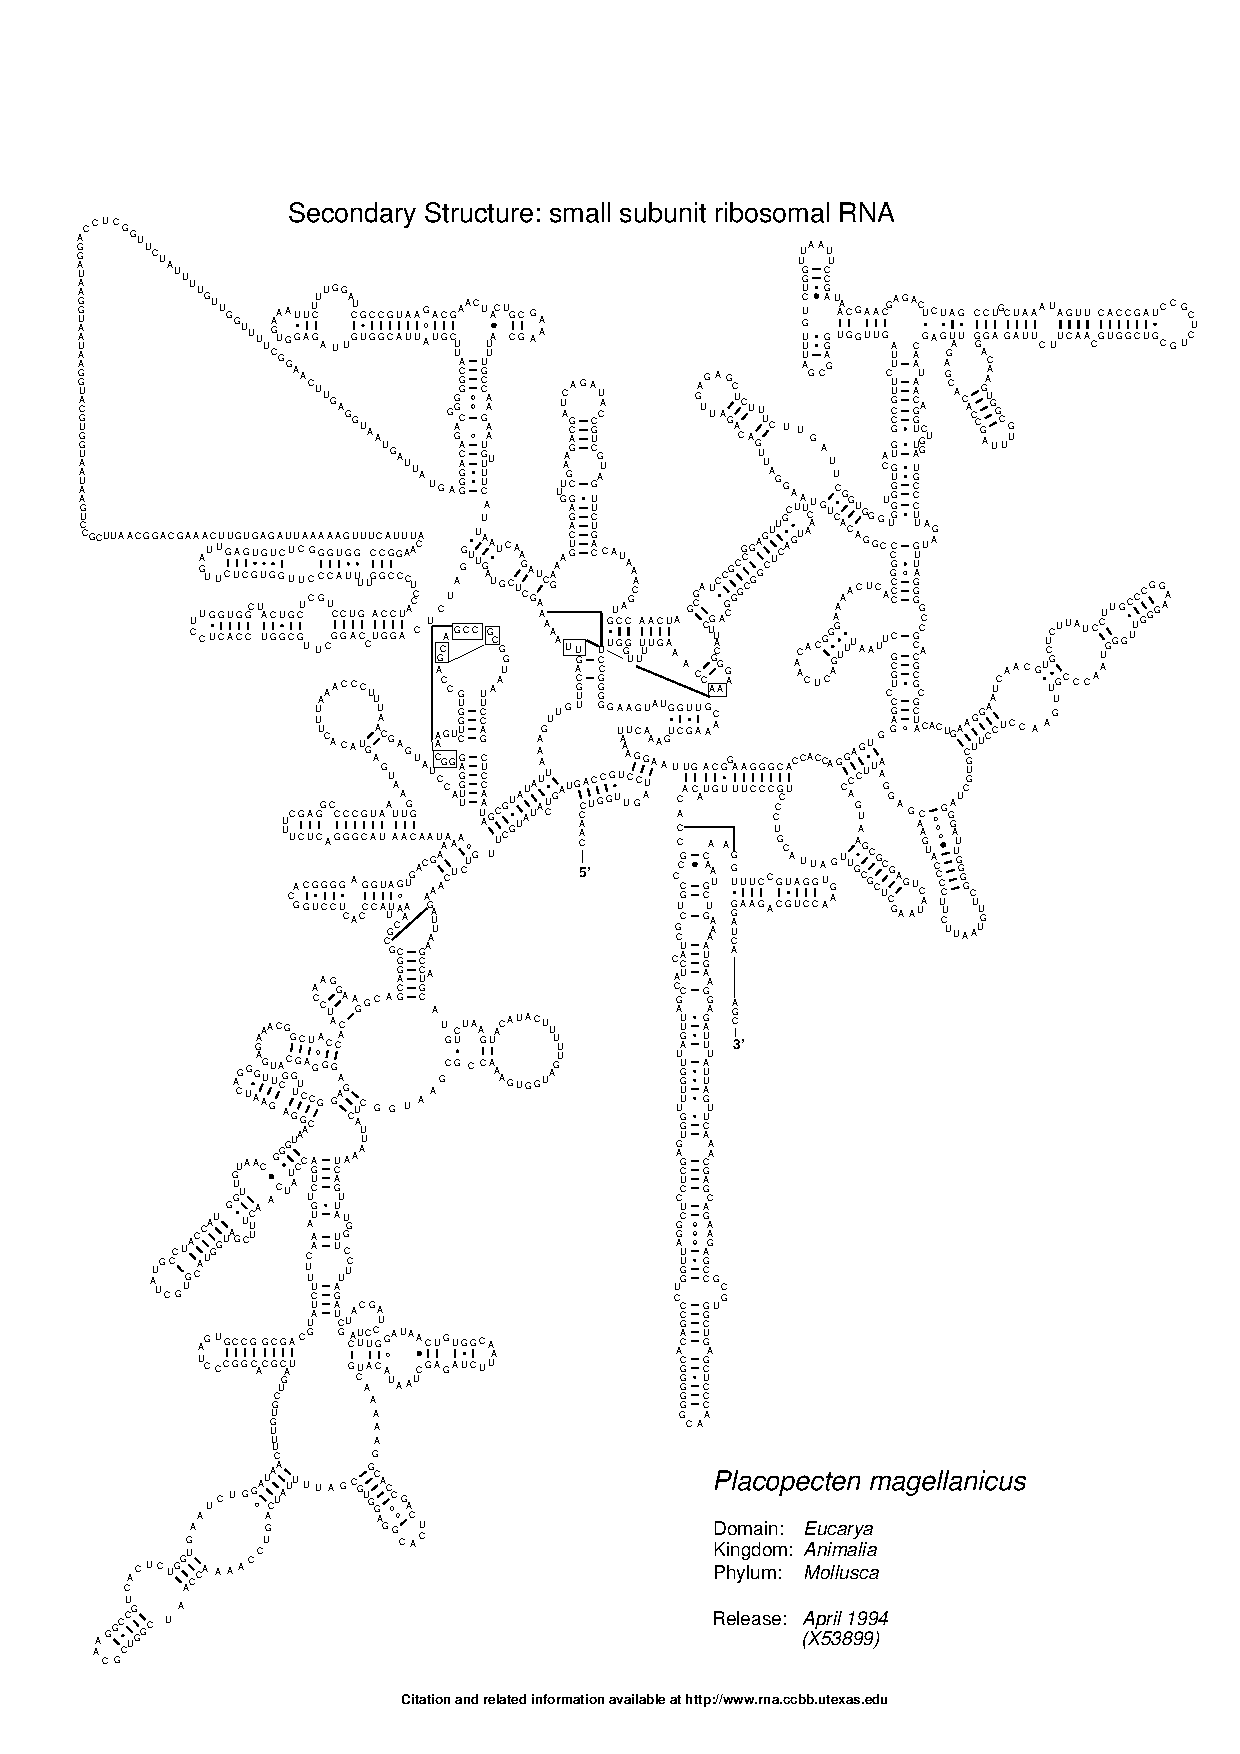
\includegraphics[width=0.45\textwidth]{../img/chyby/sea_scallop}
  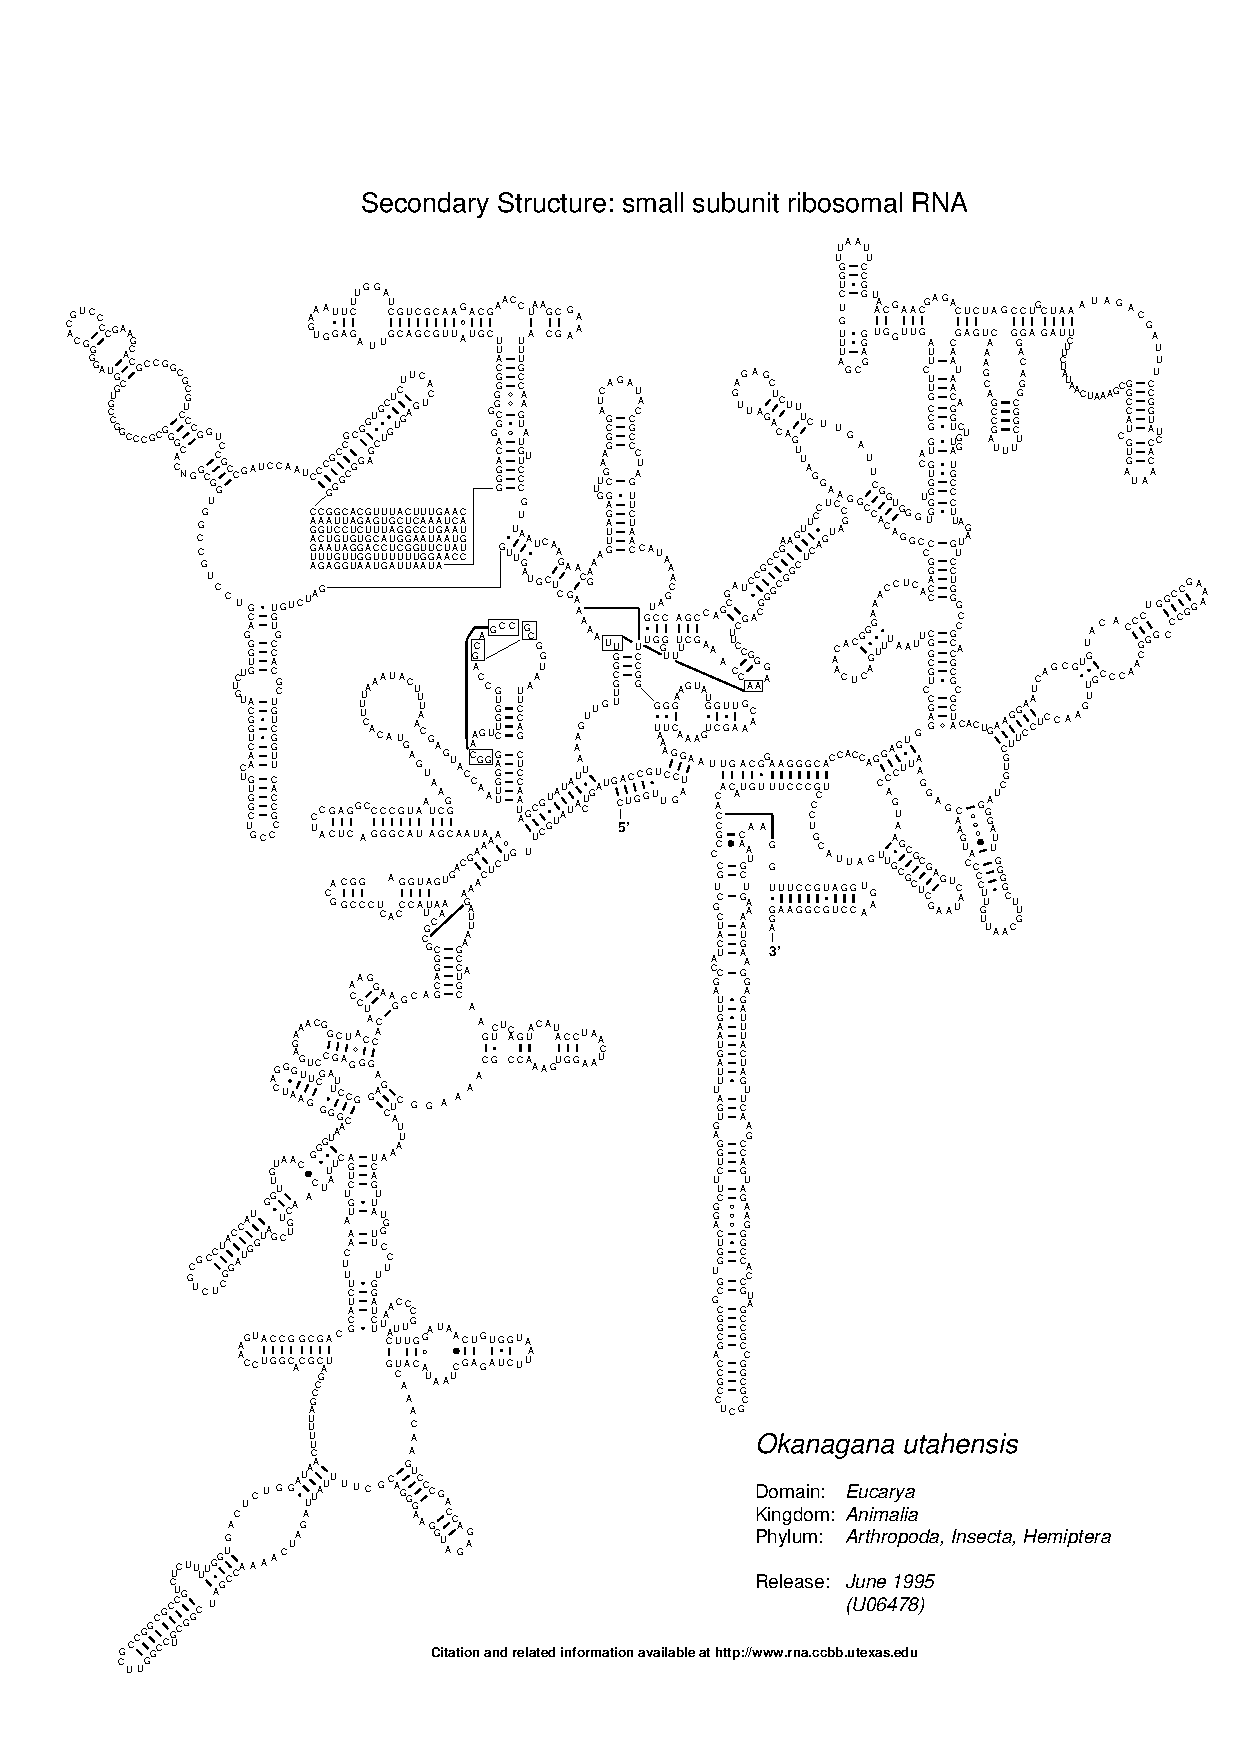
\includegraphics[width=0.45\textwidth]{../img/chyby/cicadas}
%trim=left bottom right top
  %\centering
  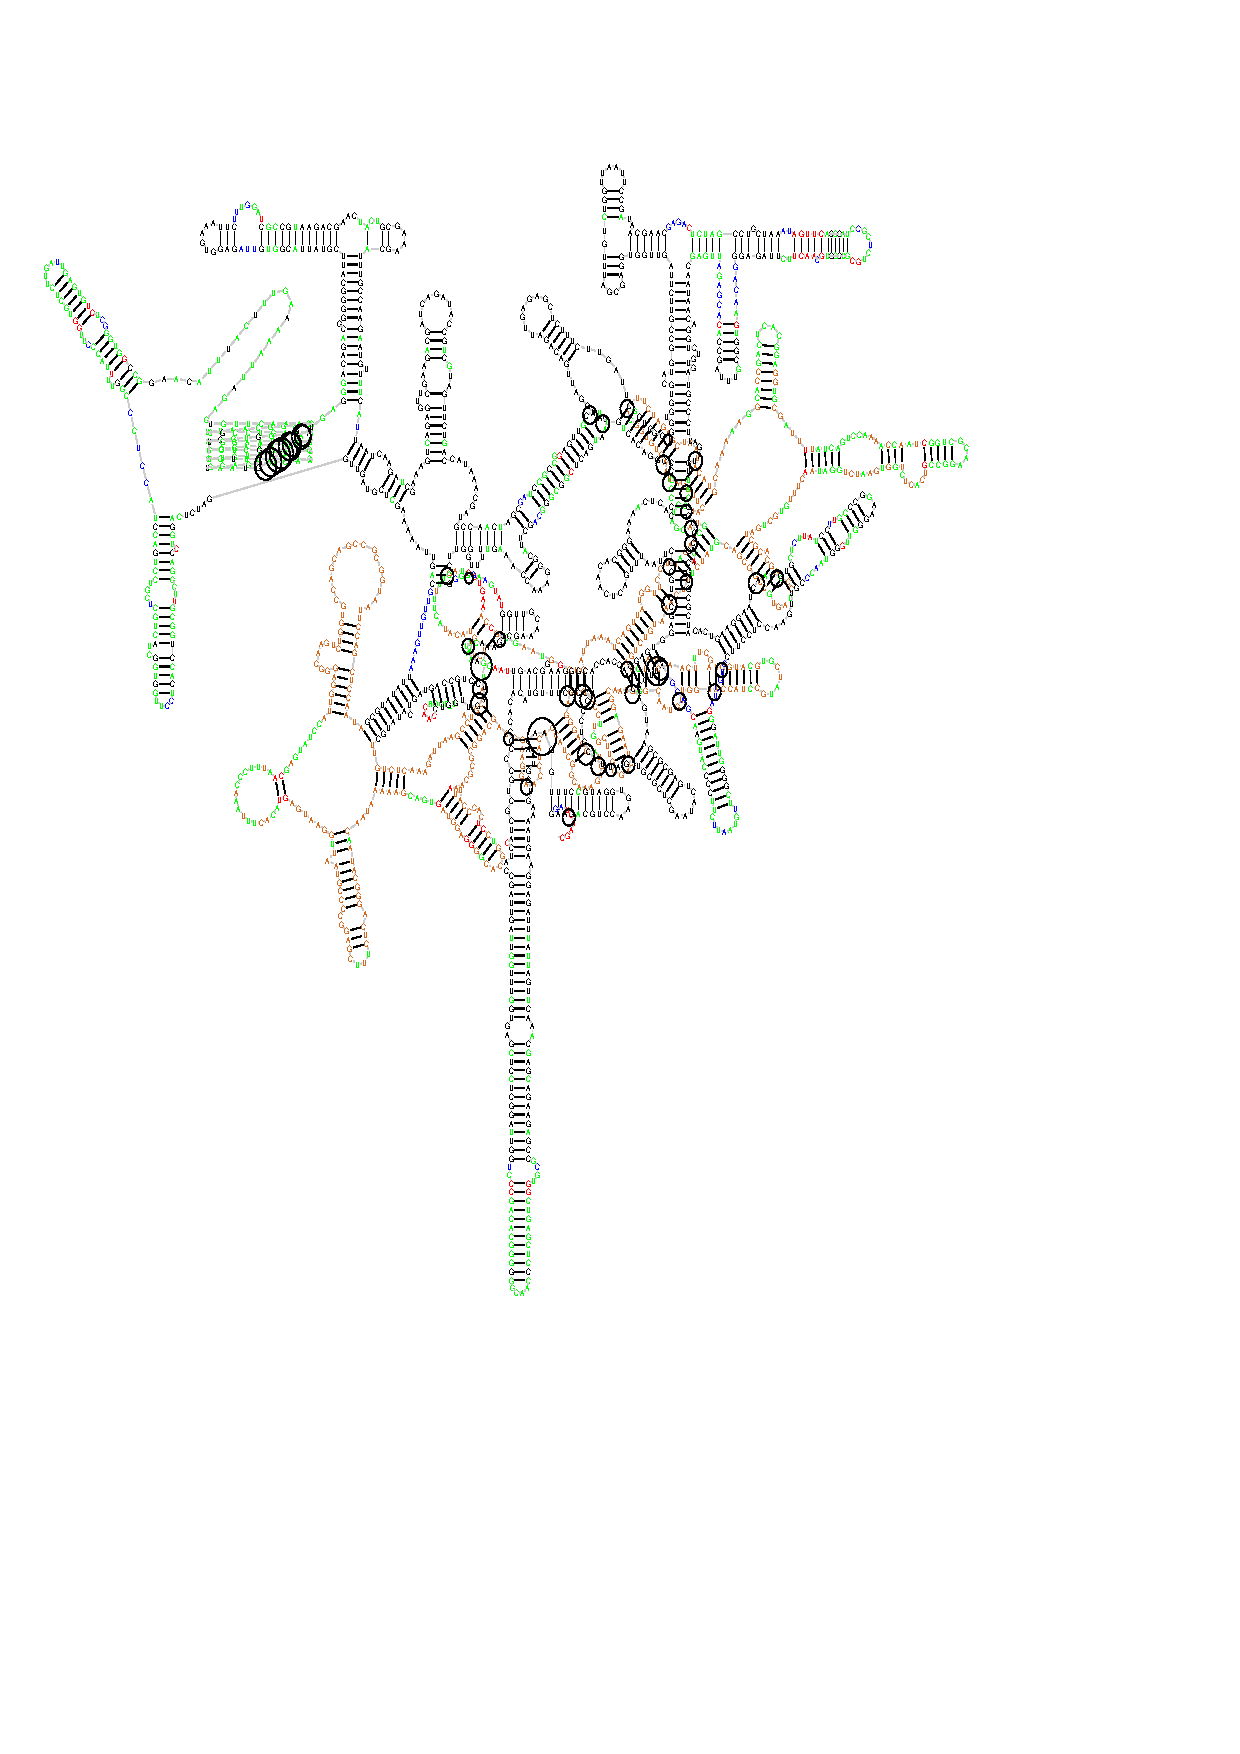
\includegraphics[clip, trim=0.5cm 7cm 4cm 2cm,width=0.45\textwidth]{../img/chyby/cicadas-sea_scallop}
  \caption{Chyba pri otacani kvoli prekreslovaniu multibranch loopy}
  \label{obr:chyba_rotacia_multibranch}
\end{figure}









